% !TEX root = presentation.tex
\section{Introduction}
\subsection{Test Suite Effectiveness}
\frame{\frametitle{Test Suite Effectiveness}
  \begin{itemize}
    \item An effective test suite is \textit{``\ldots one that is capable of \alert{detecting all real bugs}''}~\footcite{Wey93}.
    \item Can measure \alert{code coverage} (e.g., branch, statement, path) being exercised by a test suite~\footcite{ZHM97}
    \item A more \alert{effective} determination of test suite effectiveness is \alert{mutation testing}.
  \end{itemize}
}

\subsubsection{Supporting Mutation Testing}
\frame{\frametitle{Supporting Mutation Testing}
  \begin{itemize}
    \item \textbf{Competent Programmer Hypothesis}~\footcite{ABD+79}: developers write software that is \alert{nearly correct}.
    \item \textbf{Coupling Effect Hypothesis}~\footcite{Off92}: a large percent of \alert{complex faults} can be detected if all the \alert{simple faults} can be detected.
    \item Together these two hypothesis strengthen:
    \begin{itemize}
      \item The use of \alert{small/single changes} for mutation operators.
      \item Why mutation testing is \alert{adequate} for evaluating test suite effectiveness.
    \end{itemize}
  \end{itemize}
}

\subsection{Mutation Testing Overview}
\frame{\frametitle{Mutation Testing Overview}
  \begin{figure}[!tb]
    \centering
    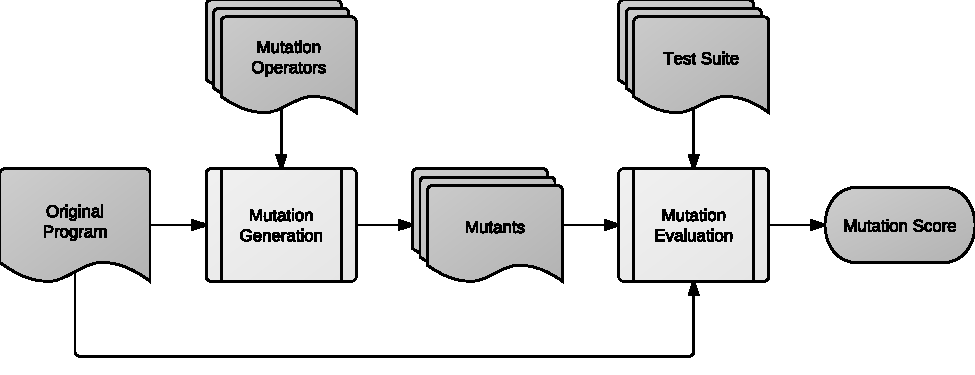
\includegraphics[width=\textwidth]{../thesis/figures/mutation_testing_overview.pdf}
    \caption{The mutation testing process.}
    \label{fig:mutation_testing_overview}
  \end{figure}
  \hrule
  \vspace{5mm}
  \begin{equation}
    \textit{$\text{mutation score} = \frac{\text{killed mutants}}{\text{total mutants} - \text{equivalent mutants}}$}
    \label{equ:mutation_score}
  \end{equation}
}

\subsubsection{Mutation Operator Example}
\frame{\frametitle{Mutation Operator Example (\textit{ROR})}
  \begin{figure}[!tb]
    \centering
    \begin{minipage}{4.75cm}
      \centering
      \footnotesize{\textbf{Original Program}}
      \lstinputlisting[language=Java, literate={>}{{\textcolor{red}{>}}}{1}]{../thesis/listings/mutation_example.java}
    \end{minipage}
    $\xrightarrow{\textit{ROR}}$
    \begin{minipage}{4.75cm}
      \centering
      \footnotesize{\textbf{Mutant Program}}
      \lstinputlisting[language=Java, literate={>}{{\textcolor{red}{<}}}{1}]{../thesis/listings/mutation_example.java}
    \end{minipage}
    \caption{Example application of the \alert{Relational Operator Replacement \textit{(ROR)}} method-level mutation operator.}
    \vspace{2mm}
    \hrule
    \label{fig:ROR_mutation}
  \end{figure}
  \begin{itemize}
    \item Replaces a relational operator (i.e., \texttt{>}, \texttt{>=}, \texttt{==}, \texttt{!=}, \texttt{=<} or \texttt{<}) with another type of relational operator.
  \end{itemize}
}

\subsubsection{Method-Level Mutation Operators}
\frame{\frametitle{Method-Level Mutation Operators}
  \scriptsize
  \begin{table}[!tb]
    \centering
    \rowcolors{2}{gray!30}{gray!20}
    \begin{tabular}{|l|l|}
      \hline
      \rowcolor[RGB]{150,160,240}
      \textbf{Operator} & \textbf{Description} \\
      \hline \textit{AOR} & Arithmetic Operator Replacement \\
      \hline \textit{AOI} & Arithmetic Operator Insertion \\
      \hline \textit{AOD} & Arithmetic Operator Deletion \\
      \hline \textit{ROR} & Relational Operator Replacement \\
      \hline \textit{COR} & Conditional Operator Replacement \\
      \hline \textit{COI} & Conditional Operator Insertion \\
      \hline \textit{COD} & Conditional Operator Deletion \\
      \hline \textit{SOR} & Shift Operator Replacement \\
      \hline \textit{LOR} & Logical Operator Replacement \\
      \hline \textit{LOI} & Logical Operator Insertion \\
      \hline \textit{LOD} & Logical Operator Deletion \\
      \hline \textit{ASR} & Assignment Operator Replacement \\
      \hline
    \end{tabular}
    \caption{The set of method-level mutation operators from the \textit{MuJava} mutation testing tool~\footcite{MOK05}.}
    \label{tab:method_operators}
  \end{table}
}

\subsection{Challenges in Mutation Testing Adoption}
\frame{\frametitle{Challenges in Mutation Testing Adoption}
  \begin{itemize}
    \item \alert{Hundreds or thousands} of mutants can be generated for even \alert{small} software systems.
    \item \alert{Slow industry adoption} of mutation testing due to \alert{performance/scalability} in evaluating mutants~\footcite{OU01}.
    \item Mutation testing would have to be applied \alert{frequently} during development
  \end{itemize}
}

\subsubsection{Proposed Approach}
\frame{\frametitle{Proposed Approach}
  \begin{itemize}
    \item Use \alert{machine learning} to \alert{predict} the \alert{mutation score} of source code units.
    \item Use \alert{software metrics} of the source code units as \alert{attributes} for predictions.
    \item \alert{Reduces} mutation testing \alert{cost} for software systems.
  \end{itemize}
}
